\section{BEE-VM Design}
\label{bee-vm-section}
%As mentioned before, some older HPC systems still run Linux system with kernel version incompatible with Docker runtime or any customized runtime system. 

To support \texttt{BEE} on older HPC systems that do not have Linux user namespace enabled, we design a second \texttt{BEE backend} for HPC system - \texttt{BEE-VM}, so that together with \texttt{BEE-Charliecloud} they make \texttt{BEE} support majority of the current HPC systems.
\texttt{BEE-VM} creates a VM layer on top of the host and then deploys Docker on the VM layer; as shown in \textbf{Fig. \ref{bee-backend}}. VM brings the isolation that enables us to run Docker even on a system with constraint. It utilizes Kernel-based Virtual Machine (KVM) (on by default in Linux), a hardware accelerated hypervisor, to provide bare-metal performance. As shown in \textbf{Fig. \ref{bee-vm}}, we run one VM per HPC host node and one Docker container per VM.

%For machines without KVM, we build and configure Quick Emulator (QEMU) in user space. QEMU runs on many host operating systems and on Linux, since kernel 2.6, that makes \texttt{BEE-VM} compatible with almost all HPC machines; however, QEMU without paravirtualization does introduce a significant performance penalty.

Similar to \texttt{BEE-Charliecloud}, besides running applications in isolated environment, another goal of the \texttt{BEE-VM} design is enabling two kinds of sharing, \textit{sharing via network} and \textit{sharing via storage}, between Docker container applications running on different machines. 
 
\subsection{Network Design}
The network design of \texttt{BEE-VM} mainly targets two functions: (1) \texttt{BEE} needs to remotely login and control each VM via SSH; (2) MPI needs network to share data between processes. 
%The network design of \texttt{BEE-VM} mainly targets two functions: First, we need to dynamically configure and deploy our VM and Docker container. This needs to be done automatically and remotely by \texttt{BEE}. We choose to utilize SSH for remote configuration. Also, since we are aiming at HPC application and most HPC applications require MPI, we need to dynamically compose a network for MPI communication between different computing nodes. For enabling that, we create a virtual subnet comprised of all VMs and corresponding Docker containers, so that they can communicate with each other.

%\subsubsection{Inter-VM network}
%We first discuss the network design at the VM layer. This is necessary because the Docker container will rely on the VM's network configuration for network in the container. 

In order to enable the SSH connection to the VM through the host, the hypervisor is configured to create dedicated virtual network interface card (vNIC) used for port forwarding that maps an unused port on the host to the SSH port on the VM. As for MPI, it cannot use the vNIC for SSH, since it usually uses a different (random) port for communication, so we cannot use port forwarding on a specific port. To handle this problem, we have two solutions. For a system with regular Ethernet, we create a second vNIC on each VM and connect all of them in a virtual subnet (i.e., multicast or P2P connection). We choose this over more straight forward approaches  (e.g., bridging) because this approach does not require any administrative privilege to the system. For a system with InfiniBand, we adopt Single Root Input/Output Virtualization (SR-IOV) to connect all VMs. To connect all the Docker containers together, we choose to start the Docker container in 'host network' in which all network configurations are exposed to the container, so that each container has the same connectivity as VM.



\subsection{Storage Design}
%\subsubsection{VM layer}
To share data between processes in Docker containers, we need to first build a shared filesystem between different VMs. Here, we use the Virtio feature \cite{russell2008virtio} in QEMU to map a host directory to a directory inside VMs. It only requires minimum configuration at VM boot time. Since HPC systems usually use shared filesystem (via NFS, Luster, etc.), each VM will also have the same file-sharing capability as long as they map to the same host directory. For data sharing in the Docker layer, we use the data volume mount feature in Docker to mount the shared folder inside VM to a directory in Docker. Since Docker runs as a process at the VM layer, mounting the data volume adds negligible overhead. 

%Since it does not rely on the virtual network, the whole virtual network is saved for MPI.

\begin{figure}[h]
	%\vspace*{-1em}
    \centering
    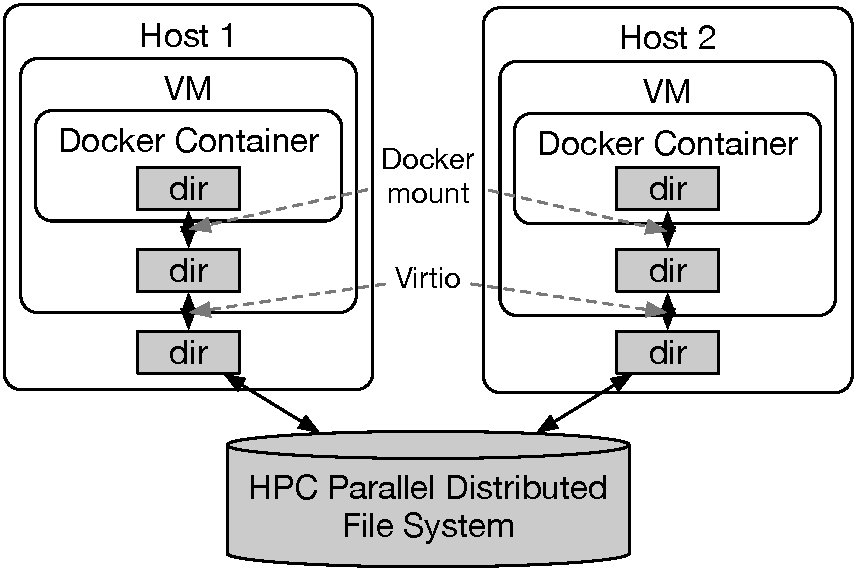
\includegraphics[width=0.4\textwidth]{figures/virtio.pdf}
    \caption{Shared Storage Design using Virtual IO}
    \label{bee-vm}
    \vspace*{-1em}
\end{figure}

%\subsubsection{Docker container layer}



\subsection{BEE-VM Deployment}
\textbf{Algorithm \ref{bee-launch}} shows the launching logic of \texttt{BEE-VM}. Before using \texttt{BEE-VM} the first time, users need to use the image builder provided by \texttt{BEE} to build the base VM image. The image is customized for \texttt{BEE-VM} that includes pre-installed softwares and settings. It only need to be done once. After that each VM will only work on a copy of the base image without any modification to the base image. During launch, \texttt{BEE-VM} first deploys VM on each HPC node (line 1 - 6). Next, the hostfile on each VM is setup in order to let each VM communicate with each other without using complicated IP addresses. The virtio storage is mounted in line 14. In the next stage, depending on what the user provides, \texttt{BEE-VM} will either pull the Docker image from public/private registries or build a new Docker image from a Dockerfile loaded into the local VM. Finally, \texttt{BEE} starts the application by launching from the first node (i.e., master node).


\begin{algorithm}
\caption{\texttt{BEE-VM} launching logic}
\label{bee-launch}
\begin{algorithmic}[1]
\REQUIRE{Pre-built QEMU Img. (only need to build once)}
\REQUIRE{Allocated host nodes: $H_1$, $H_2$,..., $H_k$}
\REQUIRE{Dockerized application (Docker image/Dockerfile)}
\REQUIRE{\texttt{BEE} configuration file (\texttt{beefile})}
\REQUIRE{Run scripts}

\FOR{i \textbf{in} 1 \textbf{to} \texttt{beefile}.num\_of\_nodes}
	\STATE \texttt{node\_i.copy\_img()}
	\STATE \texttt{node\_i.compose\_qemu\_arg(storage\_dir)}
	\STATE \texttt{node\_i.compose\_qemu\_arg(network\_conf)}
    \STATE \texttt{node\_i.start\_vm()}
\ENDFOR
\STATE \texttt{wait\_for\_all\_vm\_to\_become\_ready()}
\FOR{i in 1 \textbf{to} \texttt{beefile}.num\_of\_nodes}
\STATE \texttt{node\_i.set\_hostname()}
\FOR{j in 1 \textbf{to} \texttt{beefile}.num\_of\_nodes}
\STATE \texttt{node\_j.setup\_hostfile(node\_i.ip())}
\ENDFOR
\ENDFOR
\FOR{i in 1 \textbf{to} \texttt{beefile}.num\_of\_nodes}
\STATE \texttt{node\_i.mount\_via\_virtio()}
\ENDFOR
\FOR{i in 1 \textbf{to} \texttt{beefile}.num\_of\_nodes}
\STATE \texttt{node\_i.pull/build\_docker(beefile)}
\STATE 
\texttt{node\_i.conf\_docker\_storage(efs\_mnt)}
\STATE \texttt{node\_i.conf\_docker\_network(host\_mode)}
\STATE \texttt{node\_i.start\_docker('ssh daemon')}
\ENDFOR
\FOR{\textbf{each} \texttt{sequential run script} \textbf{in} \texttt{beefile} }
\STATE \texttt{node\_0.docker\_exec(script)}
\ENDFOR
\FOR{\textbf{each} \texttt{parallel run script} \textbf{in} \texttt{beefile} }
\STATE \texttt{node\_0.docker\_exec(mpi\_script)}
\ENDFOR

\end{algorithmic}
\end{algorithm}
